\speciestitle{Water Vapor}{H\cs2O}{H2O}{
\item[Useful range:] 316\,--\,0.001\,hPa
\item[Contact:] Alyn Lambert (stratosphere/mesosphere),
  \email{alyn.lambert@jpl.nasa.gov} \\
  William Read (troposphere), \email{william.g.read@jpl.nasa.gov}}

\subsection{Introduction}

The standard water vapor product is taken from the 190-GHz
``\texttt{CorePlusR2}'' retrieval. The vertical grid for H\cs2O is: 12
levels per decade change in pressure (LPD) for 1000\,--\,1 hPa, 6\,LPD
for 1.0\,--\,0.1\,hPa, and 3\,LPD for 0.1\,--\,10\cp{$-$5}\,hPa. The
horizontal grid is every 1.5\degsym along the orbit track.  H\cs2O is
unusual among MLS products in that it is assumed that the logarithm of
the volume mixing ratio (VMR), and not mixing ratio itself, varies linearly
with log pressure; however, H\cs2O, like the other MLS constituents is
retrieved in VMR (not $\log$ VMR). Vertical and horizontal interpolations of
H\cs2O should be performed linearly on the logarithm of the H\cs2O
concentration (VMR). The concentration of H\cs2O in the MLS files are unitless,
VMR, in the Level 2 Geophysical Product (L2GP) files; however, its
concentration is quite low in the upper atmosphere and it is more convenient
to express its concentration in parts per million volume (ppmv =
VMR$\times 10^{6}$), a unit commonly used to describe its features in this
section. The recommended vertical range is 316\,--\,0.001\,hPa (height
indicies, 7--49, starting at 1). The uppermost retrieved level 0.00046\,hPa
(height index 50) is not vertically resolved from the levels above it and is
more like a column measurement but may be usable for some studies. The MLS
science team should be consulted prior to using data from 0.00046~hPa level.

The MLS \thisv H\cs2O between 1000 and 383\,hPa is taken from a
retrieval of relative humidity with respect to ice (RHi) product,
converted to specific humidity using the Goff-Gratch vapor pressure over
ice equation.  This RHi retrieval is not vertically resolved, and all
levels between 1000 and 383\,hPa are assumed to have the same RHi.  See
Section~\ref{sec:StandardRHI} for more information. H\cs2O for
p$\le$0.000215\,hPa are filled with \emph{a priori} values. Validation of MLS
v2.2 water vapor is presented in \citet{ReadEtal:2007} and
\citet{LambertEtal:2007}.  This section reiterates the key information from
those studies, and updates them for \thisv.  Table~\ref{tab:H2OSummary}
gives a summary of MLS \thisv H\cs2O precision, resolution, and accuracy.

\subsection{Changes from \prevv}

A defect in \prevv and prior versions is that MLS exhibits a rather
low bias (20--50\%) at 2-3 km below the tropopause [Read et al in prep, 2020].
Another feature is that MLS shows a very small seasonal cycle at 147~hPa in
the tropics. The two issues are related. The tropopause height has a strong
seasonal cycle in the tropics and therefore the dry bias at a given height
will be modulated accordingly and acted to flatten the seasonal cycle at
147~hPa. Another issue is that the MLS H\cs2O measurement is drifting due
to aging of the instrument. A possible drift in the MLS H\cs2O was first noted
by \citet{HurstEtal:2016}. After an in depth investigation into possible
causes behind these issues, a most likely contributor is a combination of a
sideband fraction characterization error and a radiometer pointing error.
The center channels in the radiometer band (B2) that is dedicated to
measuring H\cs2O are opaque while the instrument FOV scans the stratosphere and
provides a temperature measurement of the stratosphere. Long term measurements
show an unexpected offset relative to what we believe is the stratospheric
temperature is and also shows a drift. Assuming that the stratospheric
temperature is known (available from the 118~GHz radiometer) and is not
drifting apart from atmospheric changes, then a new sideband fraction and
drift can be charaterized from the opaque channels in B2. The analysis
suggests that 190 GHz radiometer lower sideband fraction is 6.85\% too low
and has drifted ~1\% during the mission lifetime. Implementing these changes
helped resolve another inconsistency we had with the 190~GHz. Using the H\cs2O
linewidth to retrieve pointing e.g. tangent pressure, differed from that from
the 118~GHz radiometer which uses O\cs2 by 250m. Applying the sideband
correction reduced this inconsistency to 70m which is within the measured
uncertainty of the radiometer pointing alignment among the different
radiometers. Therefore a 70m adjustment to the radiometer alignment is
applied. With these adjustments
the retrieved ptan from the 190~GHz (CorePlusR2) is now consistent within ~20m
of that retrieved from the 118 and 240~GHz (CorePlusR3) and is retrieved
operationally now. These changes have helped to mitigate the large dry bias
2--3~km below the tropopause and consequently, increased the seasonal cycle
of the 147~hPa H\cs2O in the tropics. These changes have helped to reduce
biases and drifts between the 190~GHz and the standard product ozones.

Another improvement to the H\cs2O retrieval is using a line by line radiative
transfer model to calculate radiances for the digital autocorrelator channels
(128, 100~kHz channels centered on the H\cs2O line) instead of using a
linear approximation of the model. This change will properly account for non
linearities in the signal dependence on the H\cs2O concentration. Some
adjustments were made to the \emph{a priori} precision and smoothing to
produce positive precisions and potentially make
the product useful up to 0.001~hPa. The retreival range for H\cs2O
is raised to 0.00046~hPa in \thisv.

The median daily quality for v4.2 declined by 4.8\% from 2010 to 2020. The
decline follows a declining trend in the radiometer system temperature that
determines the measurement signal noise that is also declining making the
goodness of fits degrade slightly. In \thisv, the decline over the same ten
year period is only 0.8\% due to incorporating a tangent pressure retrieval.

\begin{figure}
\begin{center}
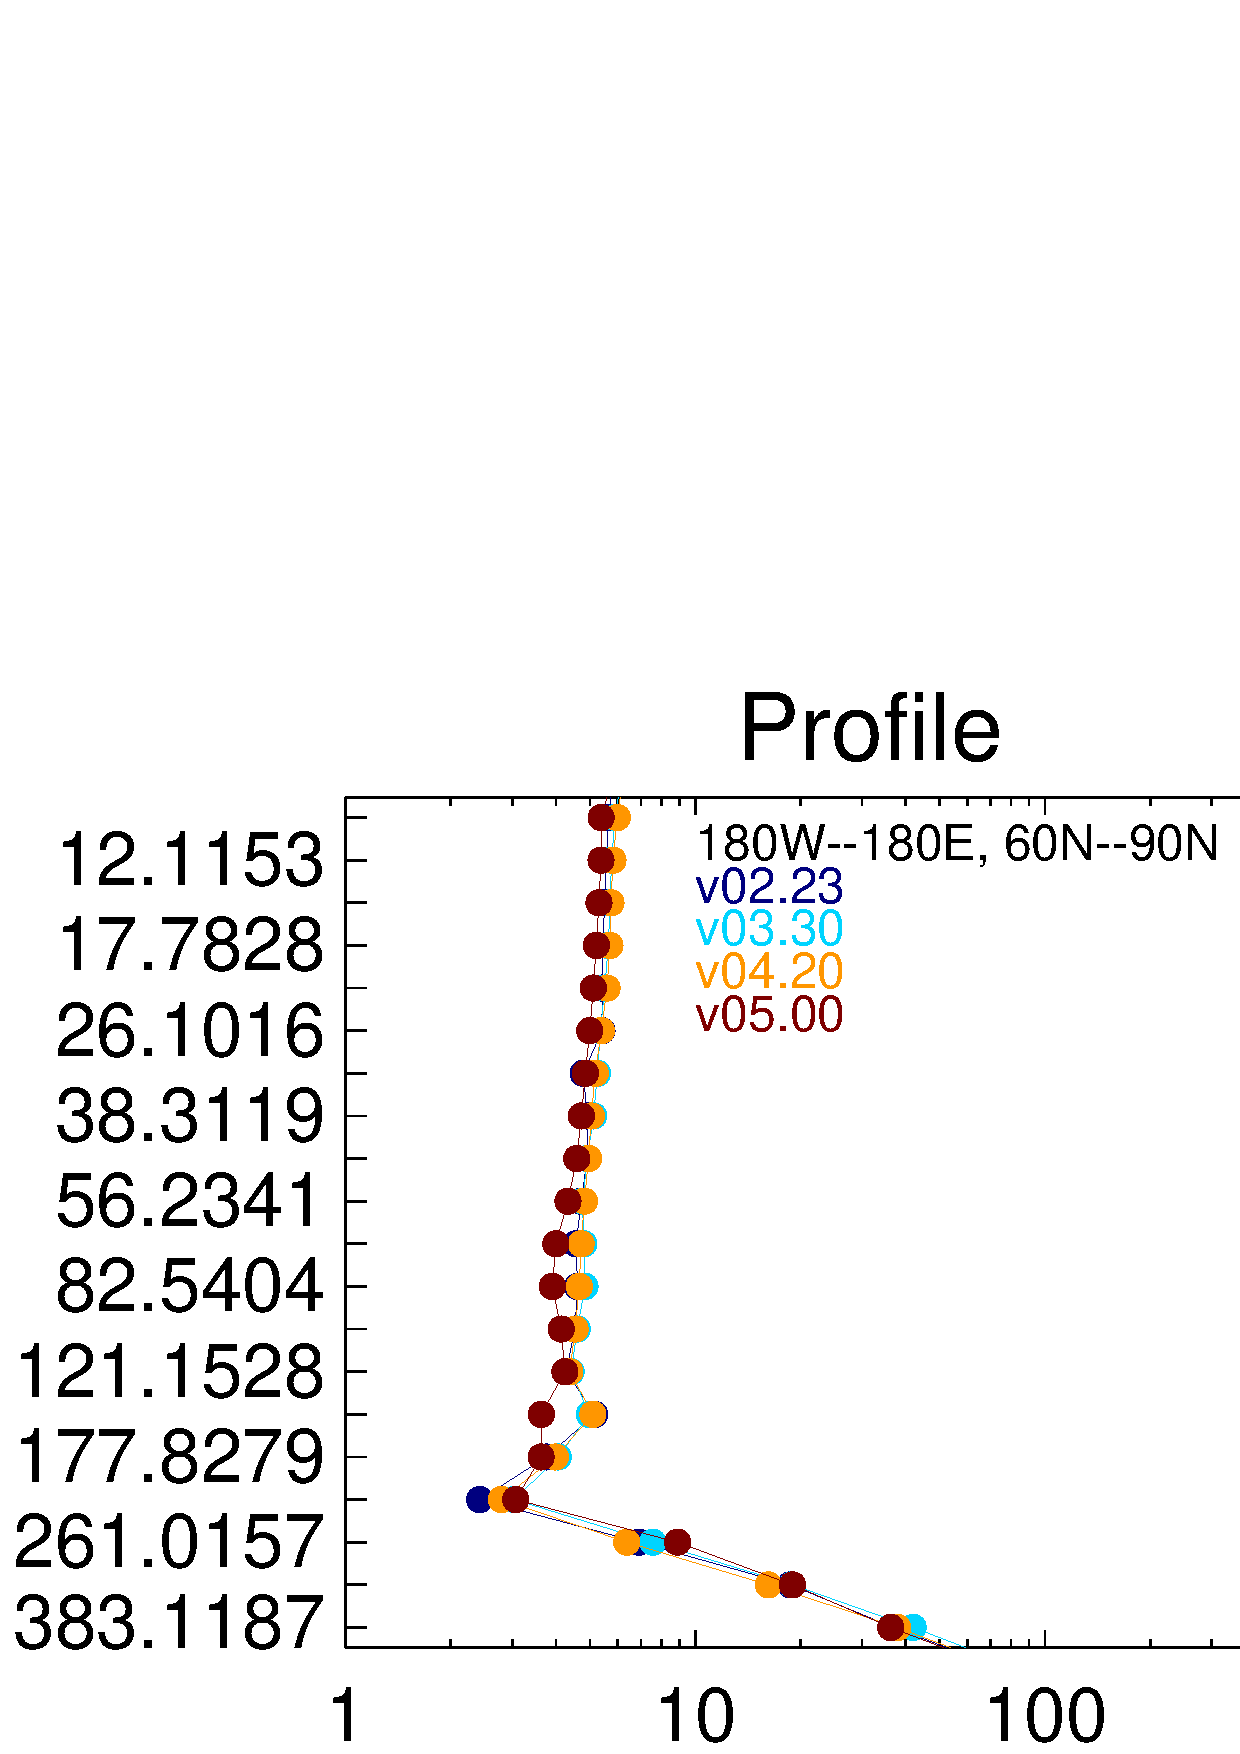
\includegraphics[width=0.8\linewidth]{figures/mls_h2o_v2-v3-v4-v5_prfl_comp_60n-90n}
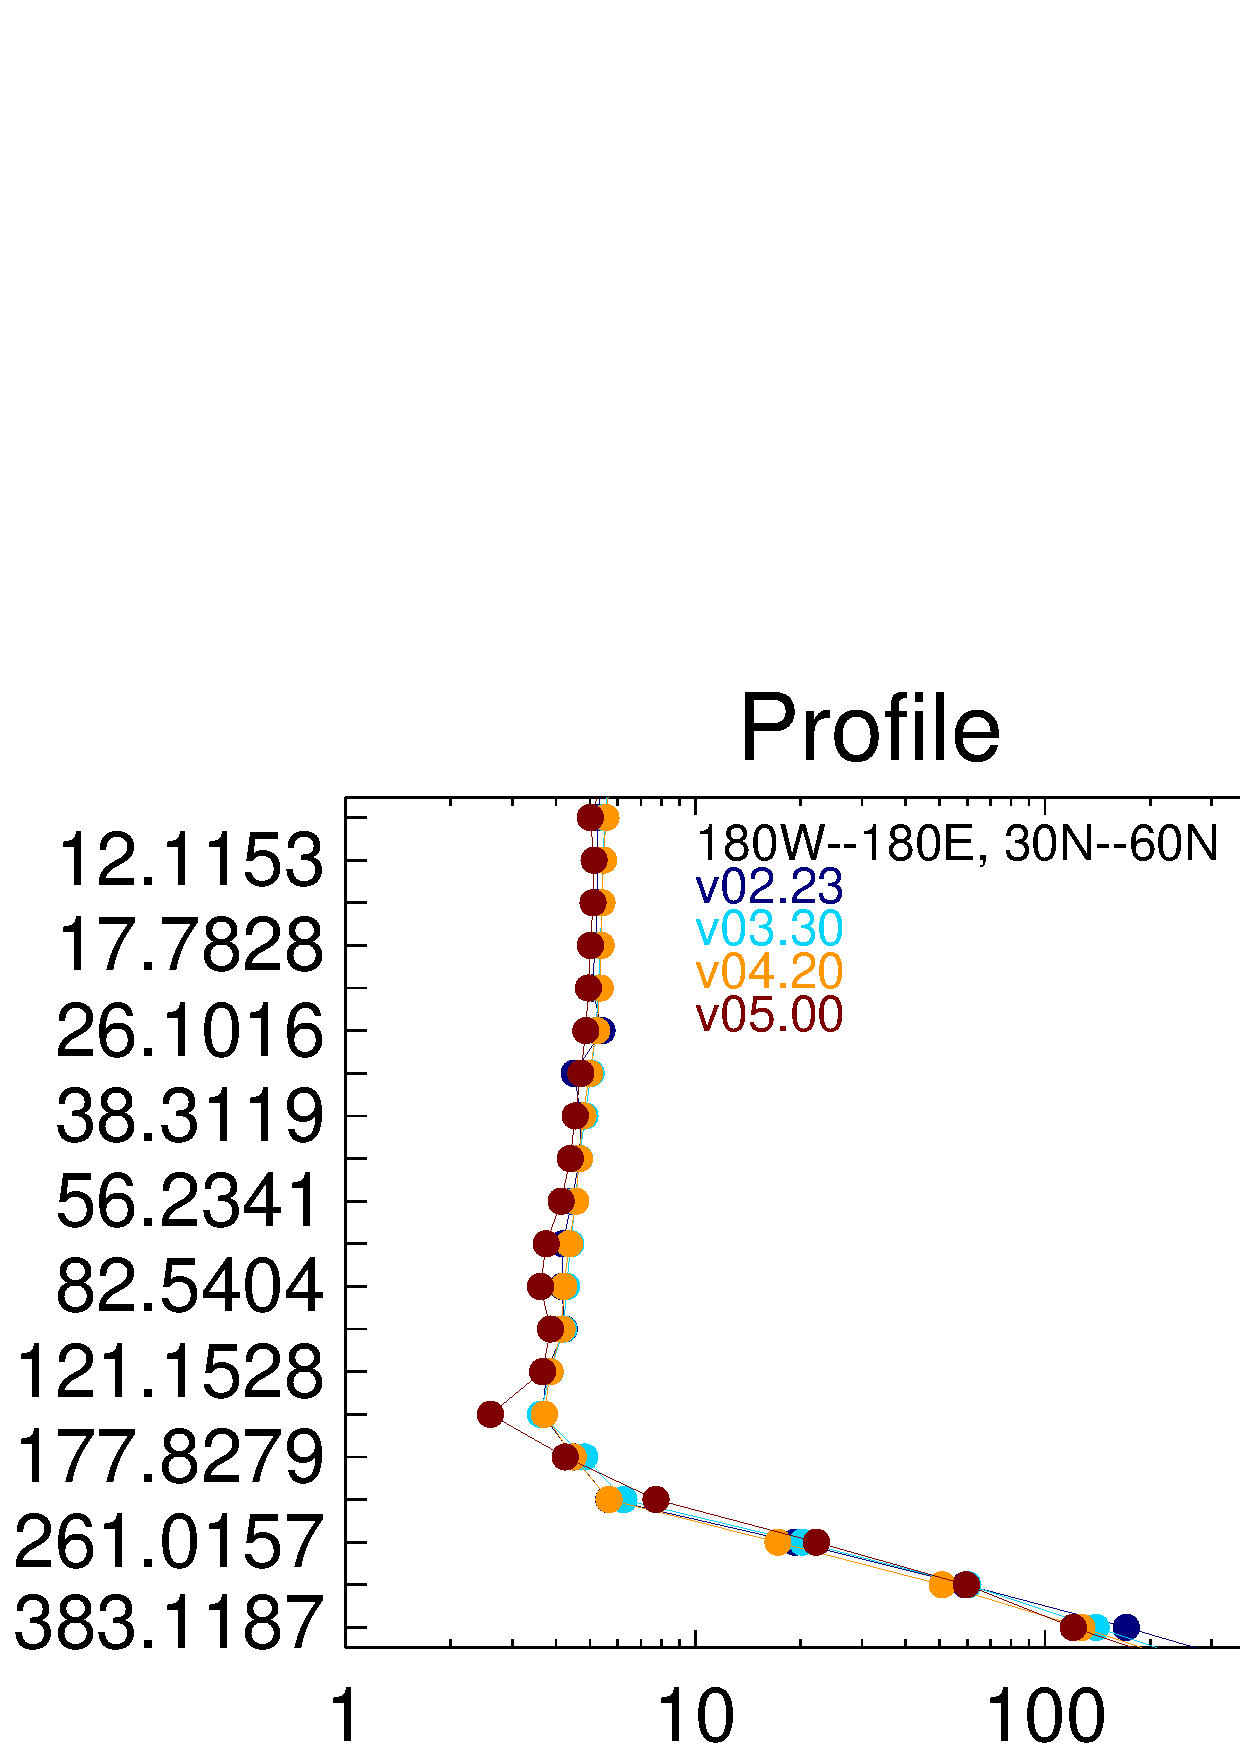
\includegraphics[width=0.8\linewidth]{figures/mls_h2o_v2-v3-v4-v5_prfl_comp_30n-60n}
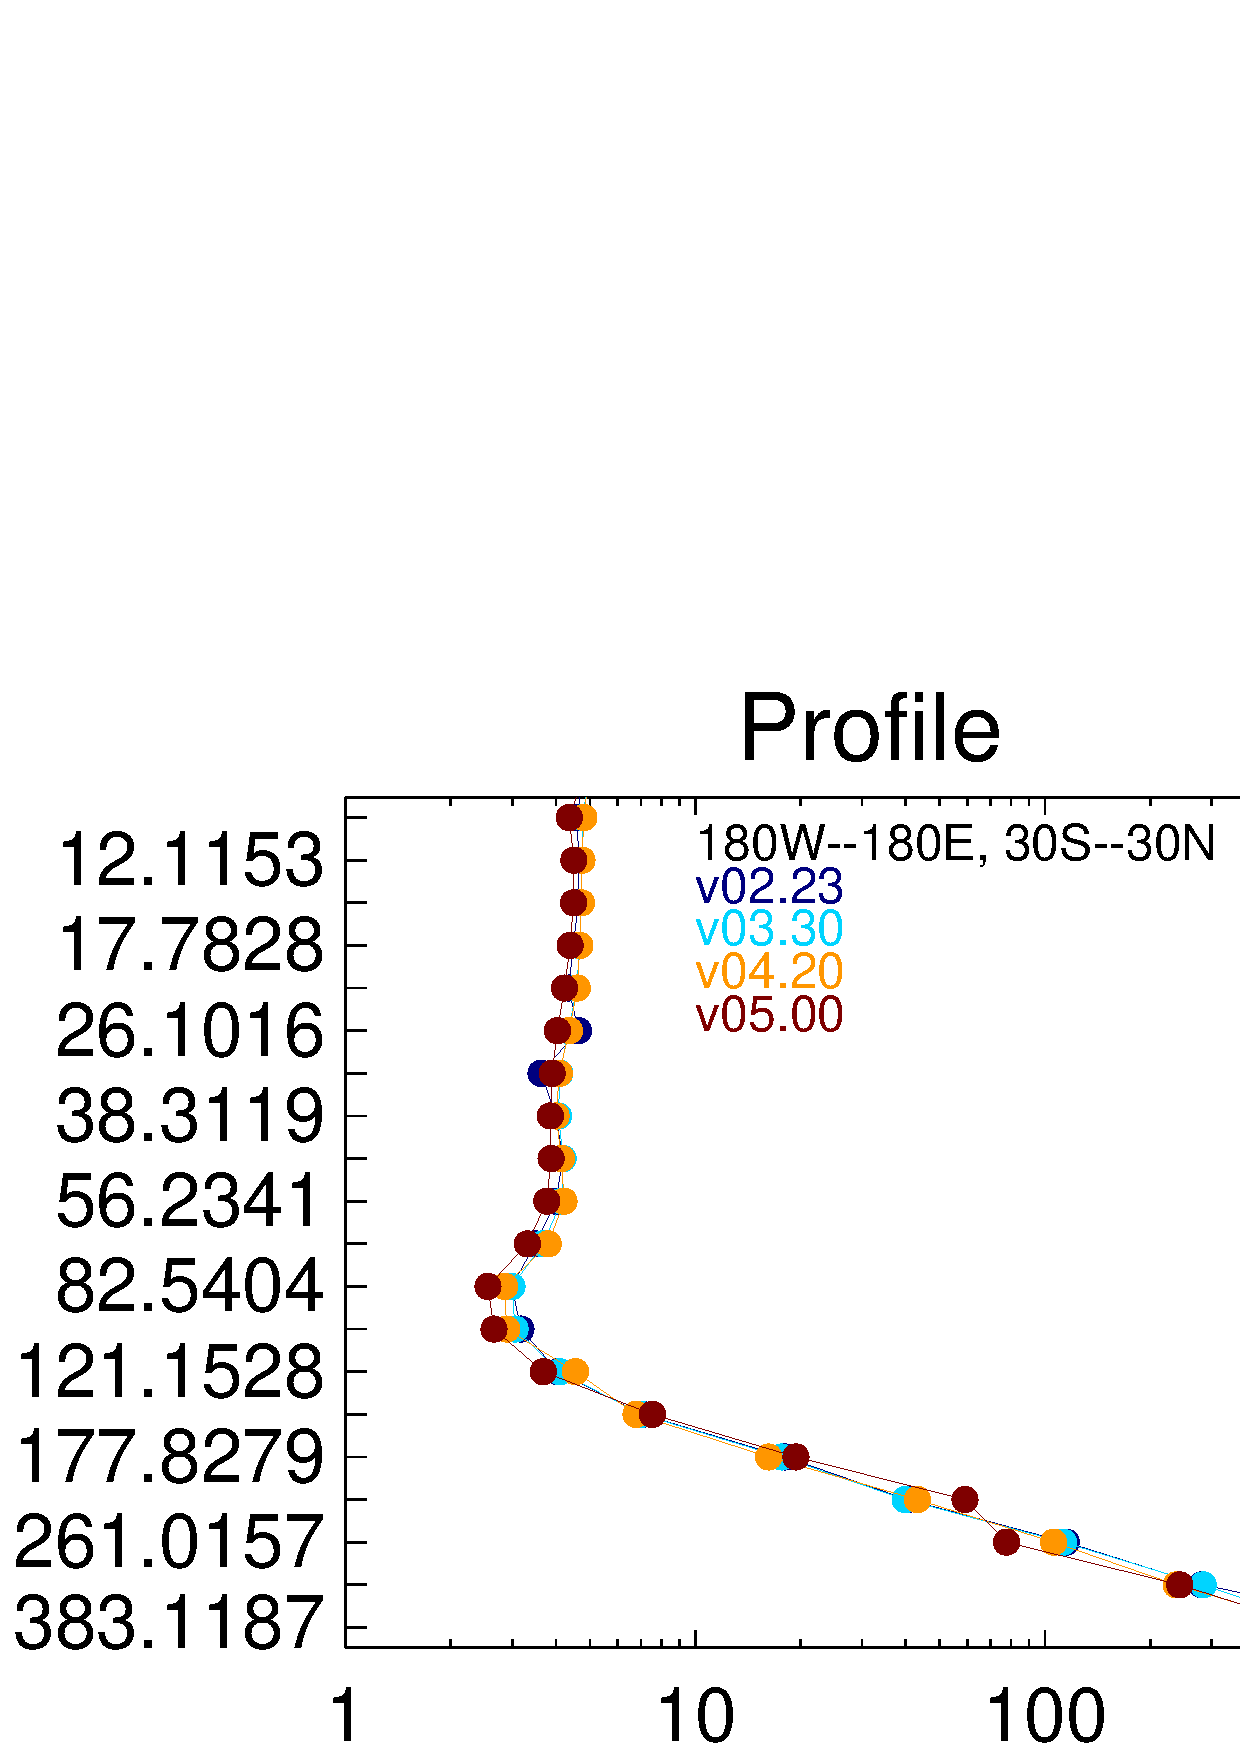
\includegraphics[width=0.8\linewidth]{figures/mls_h2o_v2-v3-v4-v5_prfl_comp_30s-30n}
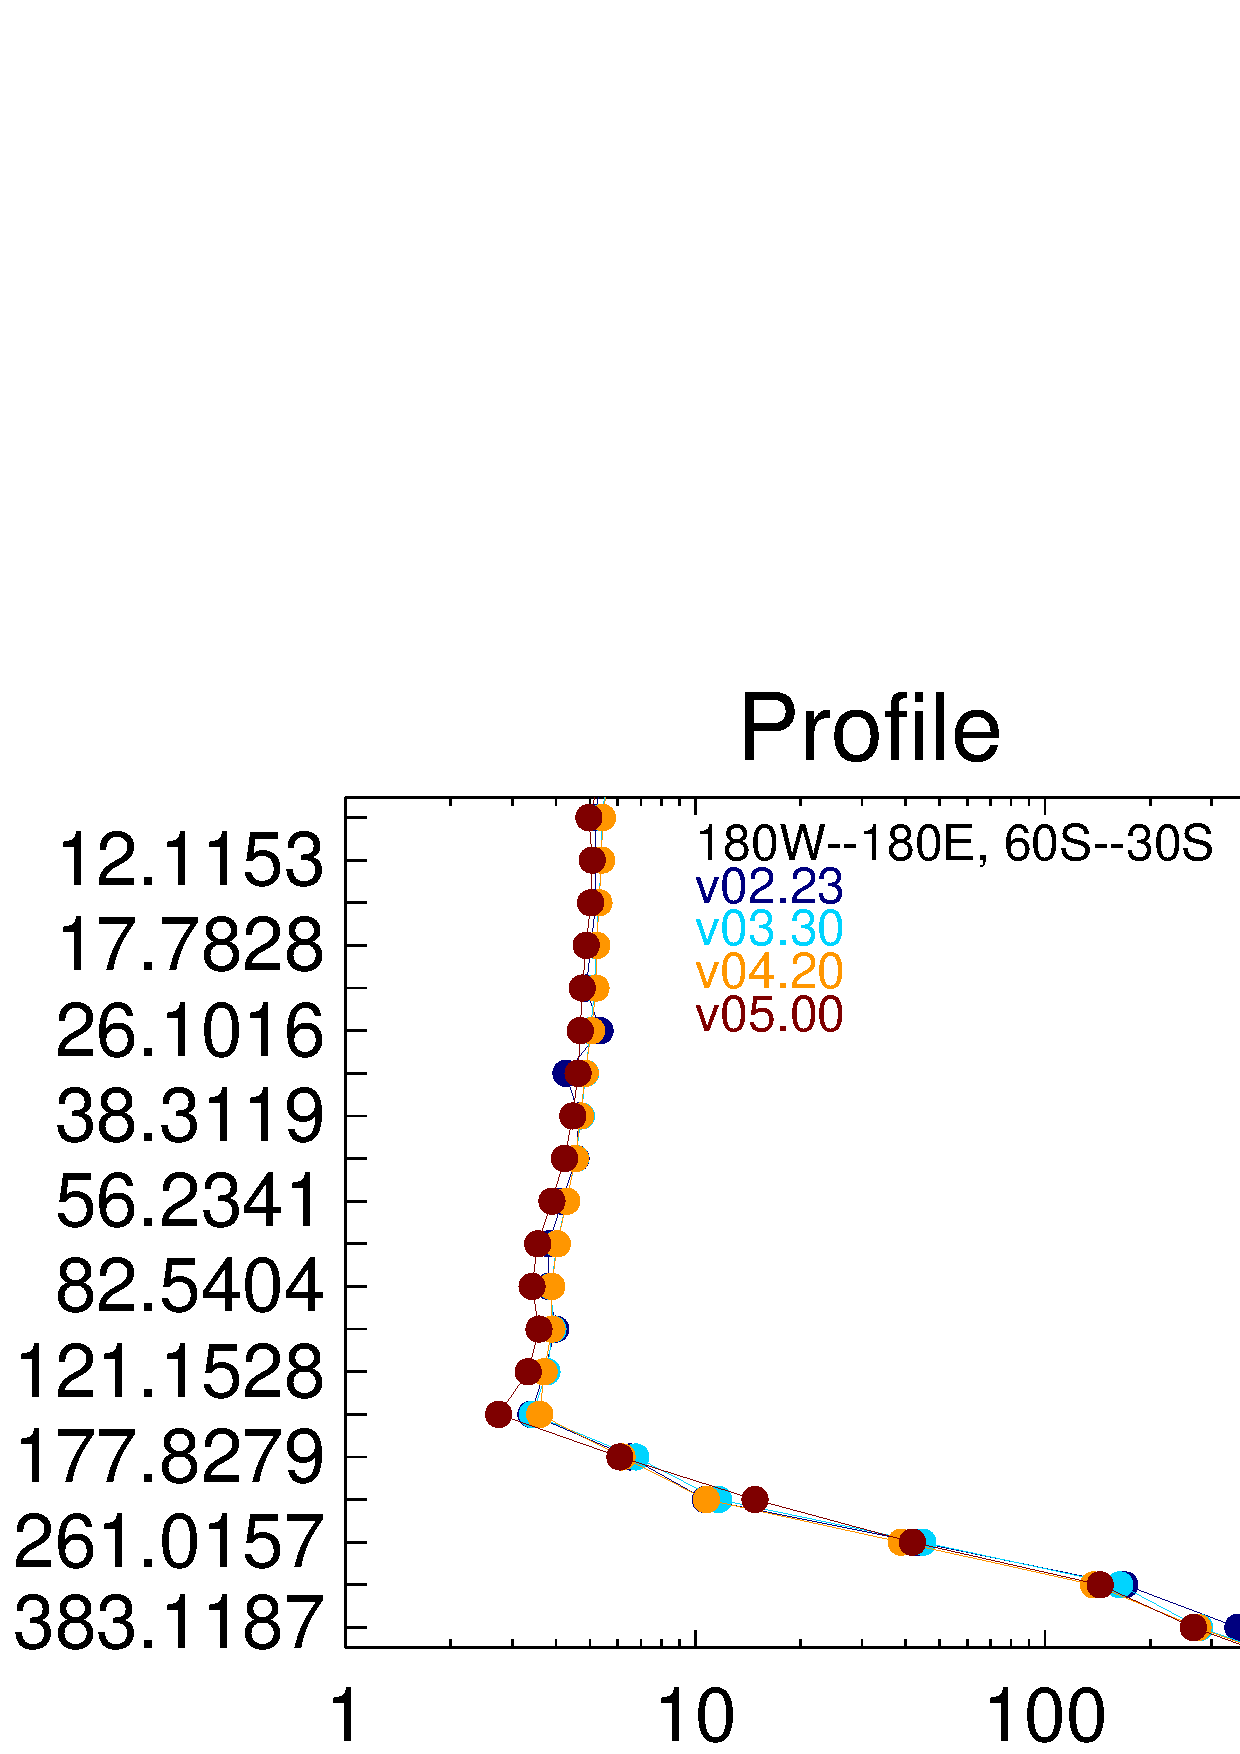
\includegraphics[width=0.8\linewidth]{figures/mls_h2o_v2-v3-v4-v5_prfl_comp_60s-30s}
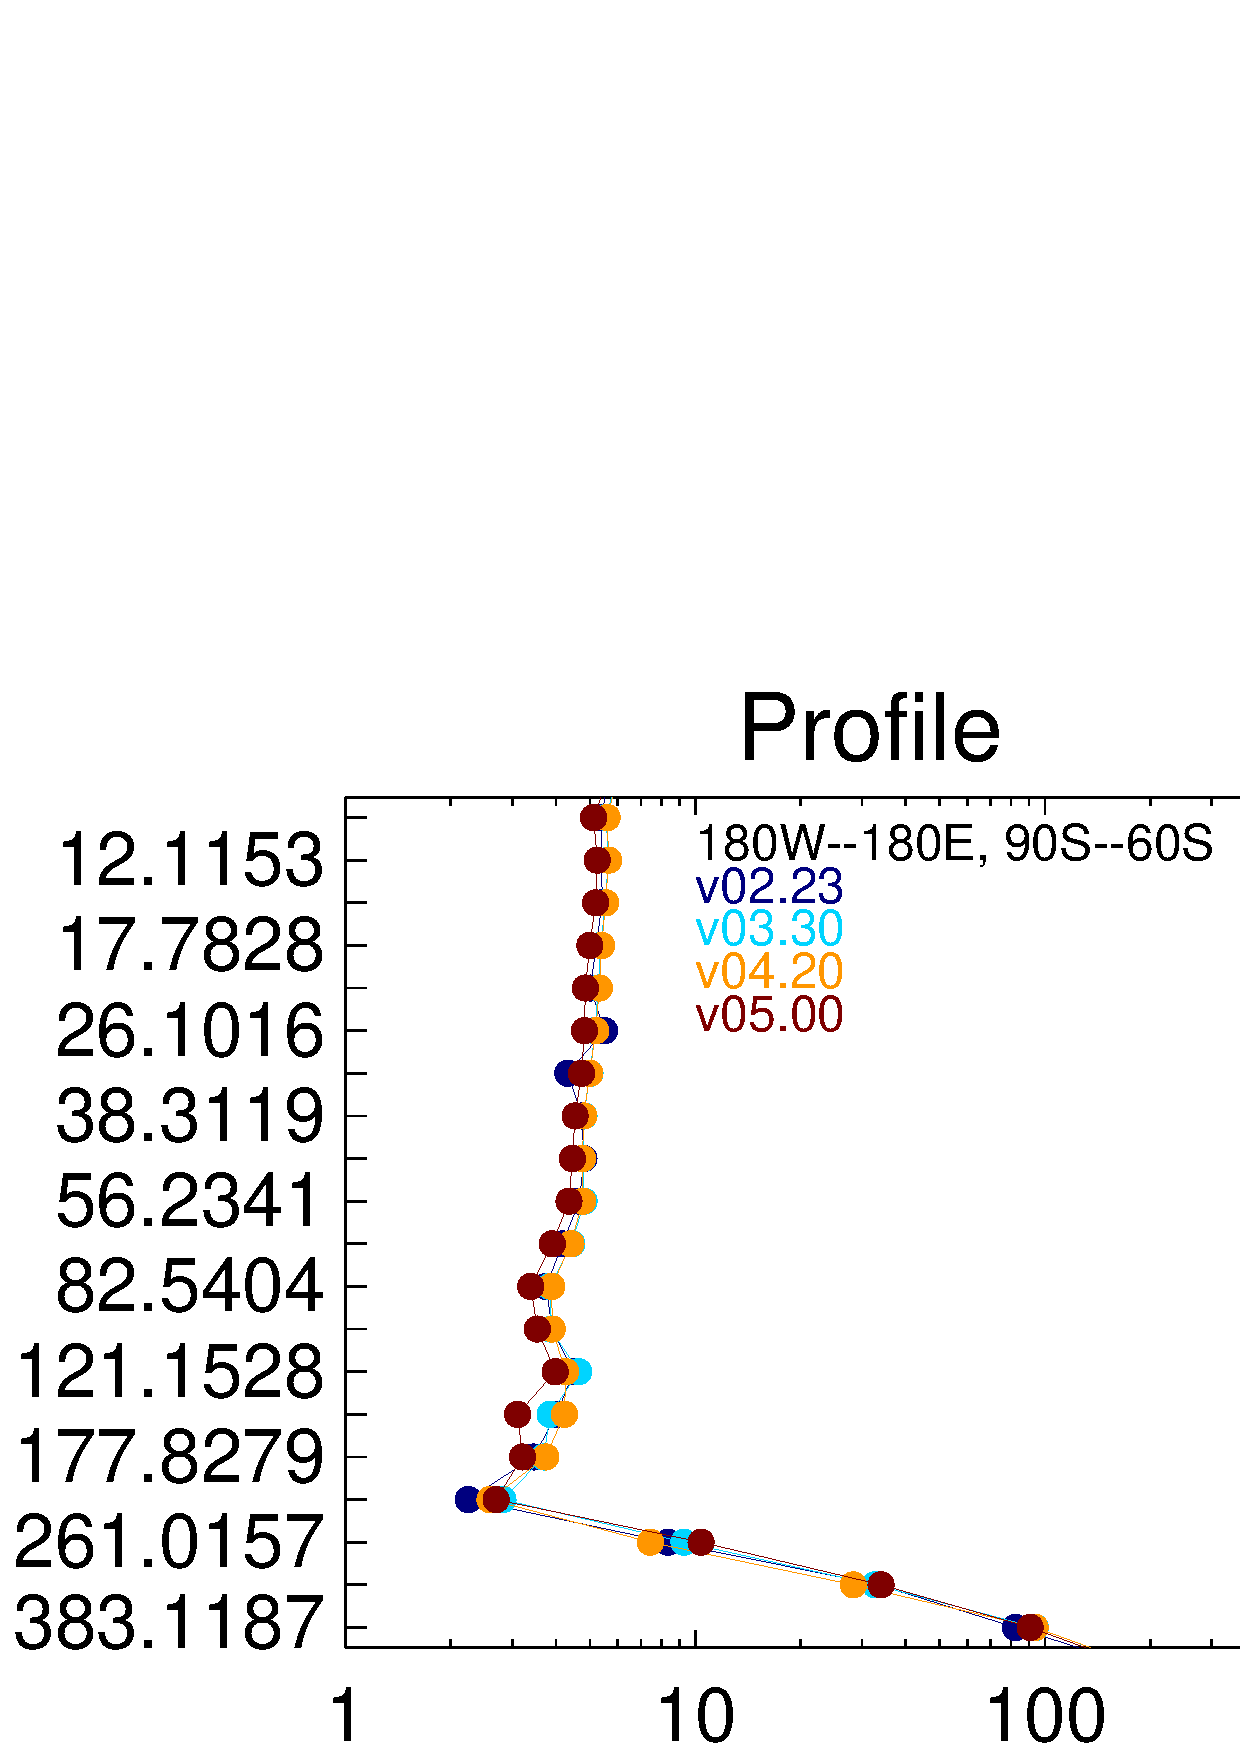
\includegraphics[width=0.8\linewidth]{figures/mls_h2o_v2-v3-v4-v5_prfl_comp_90s-60s}
\end{center}
\caption{A comparison of v2.23(blue), v3.30 (cyan), v4.20 (orange), and
  v5.00 (red) water vapor for Jan-Feb-Mar 2009 in 5 latitude bands. Other time
  periods are similar. The left panel compares mean profiles, the center
  shows the mean difference (red and green diamonds) surrounded by each
  version's estimated precision, and the right panel shows the estimated
  retrieval precision (solid and bullets), measured variability
  (dotted),  which includes atmospheric variability about the mean, and the
  \emph{a priori} precision (dashed and diamonds) profile.}
\label{fig:avgmlsprflcomptropstrat}
\end{figure}

Figure~\ref{fig:avgmlsprflcomptropstrat} compares MLS \thisv to all previous
versions starting with v2.2. The differenes are with respect to v2 which is
the product the validation paper was written about. Notable differences are
the removal of a kink in v2.2 at 32/26~hPa beginning with v3.3 caused by a
linewidth error and extending a finer grid, 12 lpd versus 6, above 22~hPa
to 1~hPa. Version 4.2 saw improvements in cloud screening and in the lower
resolution initial H\cs2O phase that is used to
initiallize values and profile shape smoothing for the final high resolution
phase. These changes improved agreement with similated data at the
316--215~hPa levels. The change in sideband fraction in v5 leads to a 5--10\%
reduction in H\cs2O in the stratosphere and above. The change in pointing
also caused by the sideband fraction change and the new estimate of the
radiometer pointing offset causes a moistening of the levels 2~km below the
tropopause. Nominally this is 147~hPa in the tropics, 215~hPa at mid-latitudes
and 261~hPa at high latitudes. The extremely low values retrieved at 215~hPa
at high latitudes seen in previous versions appear to be less dry in v5.

The handling of humidity data at pressures greater than 316\,hPa is
unchanged from v4. Text describing those changes in the v4 quality document
is repeated here. Humidity data at pressures greater
than 316\,hPa are derived from a
broad layer relative humidity retrieval (using low limb viewing MLS wing
channel radiances) similar to that obtained from NOAA operational
humidity sounders such as TOVS\@. As noted in \citep{ReadEtal:2007}, the
v2.2 retrieval at pressures larger than 316\,hPa was likely to be
\texttildelow30\% too high, based on comparisons with AIRS\@. The
accuracy of this retrieval is highly sensitive to the transmission
efficiency of the MLS optics system. In \prevv the assumed value of the
MLS antenna transmission efficiency was adjusted empirically (within the
uncertainty range established from MLS calibration) to give better
agreement with AIRS in the tropics. In \thisv the N\cs2 continuum was
adjusted only for this phase to minimize the clear sky cloud induced
radiance bias. This retrieval is used as an \emph{a priori} and profile
constraint for the humidity profile at pressures greater than 316\,hPa,
which are not retrieved in the standard H\cs2O product retrieval.

\sloppypar The third panel in Figure~\ref{fig:avgmlsprflcomptropstrat}
shows the mean
estimated single profile precision and the measured variability (which
includes instrument noise and atmospheric variability). The estimated
precisions are similar for most heights except up high 0.0046--0.00046~hPa
where the smoothing and uppermost retrieval level was changed and raised
respectively and in the upper troposphere where the estimated precision
roughly scales by the amount of H\cs2O. Higher concentrations of H\cs2O are
typically accompainied with higher values of precision. Because of the large
dynamic range of possible humidity in the upper troposphere and the non-linear
behavior of the instrument response to these concentrations is why H\cs2O
basis representation uses logarithm of concentration. Version 2
used a more coarse retrieval grid above 22\,hPa and a different value of
the H\cs2O linewidth.  Together these account for H\cs2O precision
differences at these altitudes between v2 and later versions.

\begin{figure}
\begin{center}
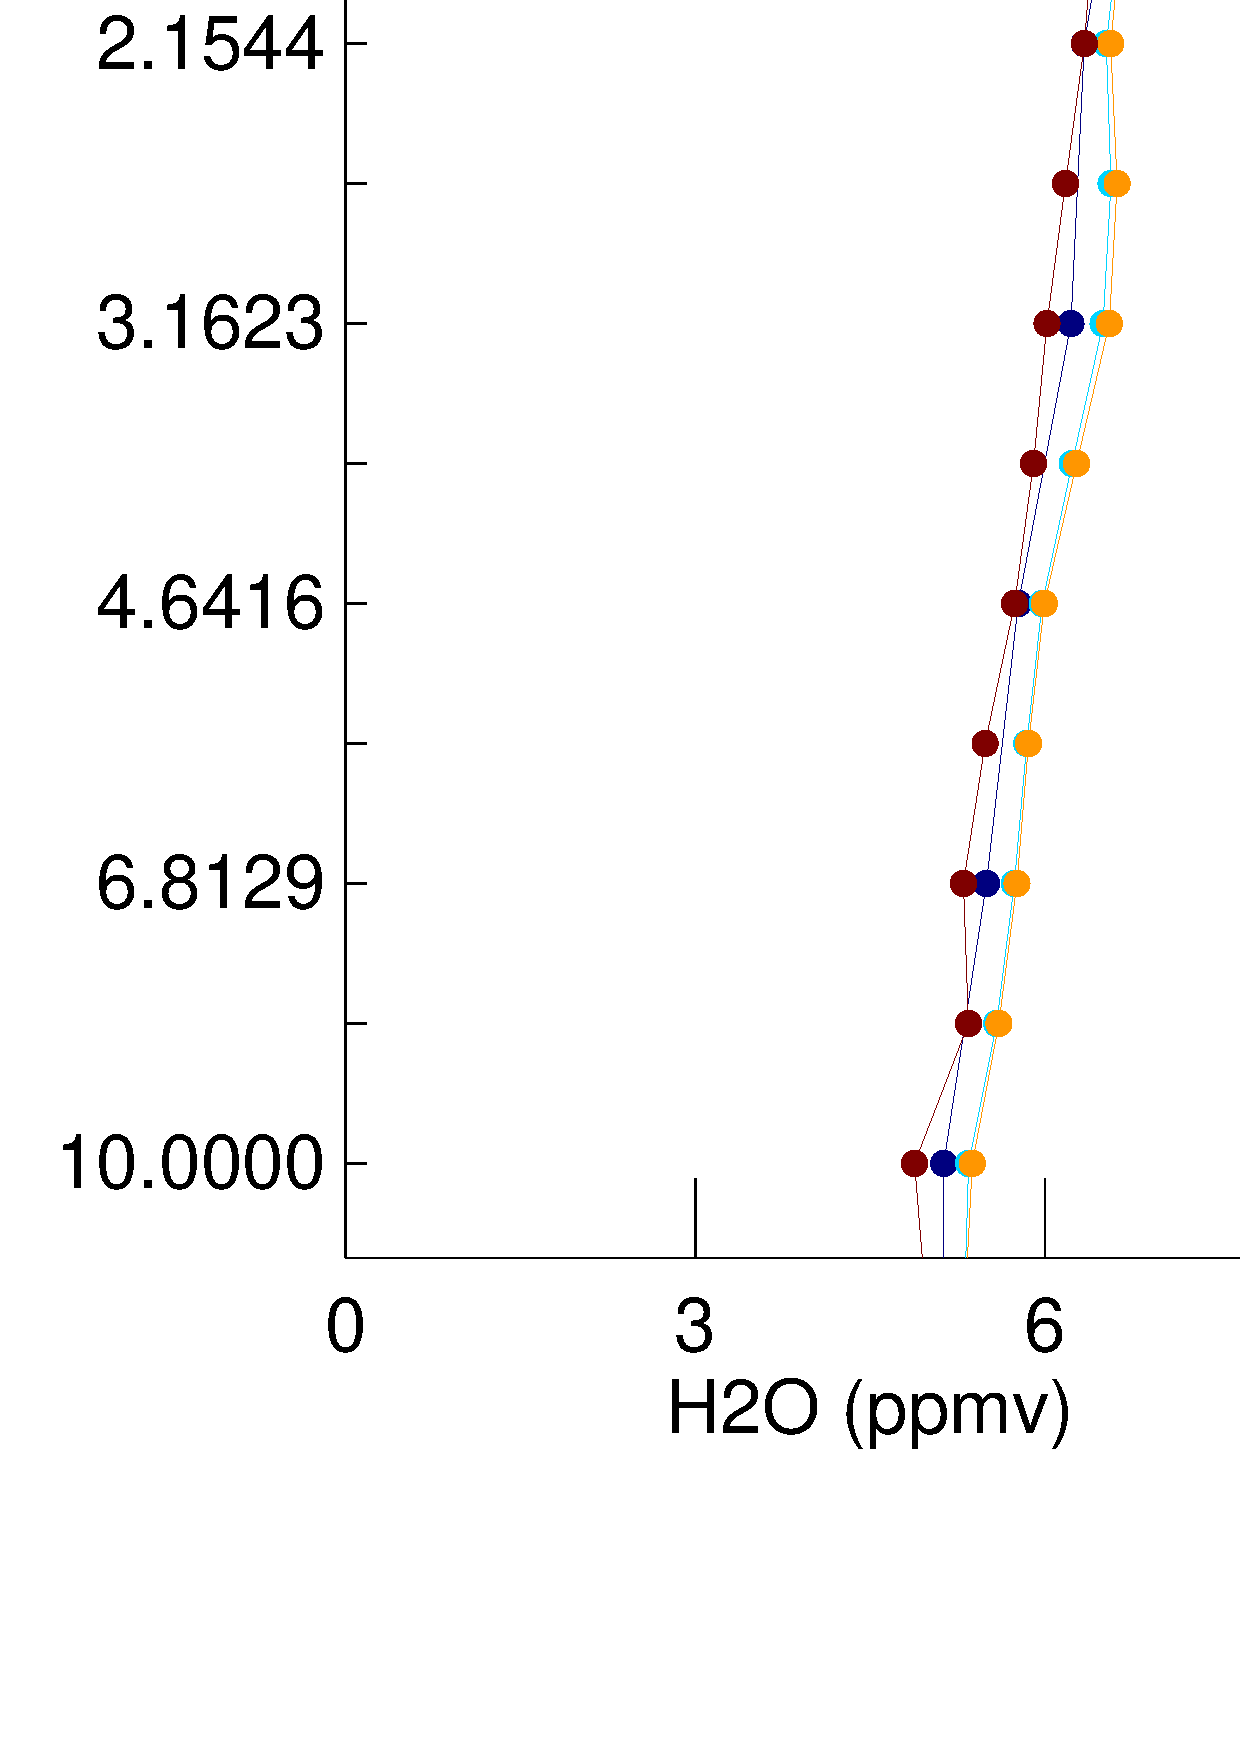
\includegraphics[width=0.8\linewidth]{figures/mls_h2o_v2-v3-v4-v5_prfl_comp_90s-90n_stratmeso}
\end{center}
\caption{An all-latitudes comparison of v2.23(blue), v3.30 (cyan), v4.20
  (orange), and v5.00 (red) water vapor for Jan-Feb-Mar 2009 showing levels
  in the middle stratosphere up to the mesosphere. Other time
  periods are similar. The left panel compares mean profiles, the center
  shows the mean difference (red and green diamonds) surrounded by each
  version's estimated precision, and the right panel shows the estimated
  retrieval precision (solid and bullets), measured variability
  (dotted),  which includes atmospheric variability about the mean, and the
  \emph{a priori} precision (dashed and diamonds) profile.}
\label{fig:avgmlsprflcompstratmeso}
\end{figure}

Figure~\ref{fig:avgmlsprflcompstratmeso} compares all versions beginning
with v02.2 to \thisv from 10~hPa to 0.0001~hPa. As expected, H\cs2O from
\thisv is lower than the other versions except v2 which had an erroneous
linewidth. Also shown is the increased \emph{a priori} precision being used
for \thisv for pressures lower than 0.0046~hPa in order to make the 0.001 and
0.00046~hPa levels usable. Using a non-linear radiative transfer model in
\thisv in place of an approximate linear model for the highly spectrally
resolved digital autocorrelator spectrometer (DACS) leads to some biases
in the uppermost levels. It is believed that
the better model being used for \thisv will produce more accurate results.

Figures~\ref{fig:avgmlsh2ozmcomp1} and \ref{fig:avgmlsh2ozmcomp2} show a
comparison of H\cs2O zonal means from v2, v3, v4, and v5 retrievals for
316\,--\,8.3\,hPa and 6.8\,--\,0.00046-hPa, respectively. In the stratosphere
v5 is usually lower than the previous versions due to the sideband adjustment.
Version 5 also shows a moist 147~hPa humidity in the tropics that becomes
a more moist 215~hPa at mid latitudes finalizing with a more moist 261~hPa at
high latitudes. In the mesosphere P$<$1~hPa, V5 is usually lower than the
previous versions but show similar structure until the top level
0.0005 (0.00046)~hPa where all other versions return the \emph{a priori},
but is actually a retrieved level in v5.

\begin{figure}
\begin{center}
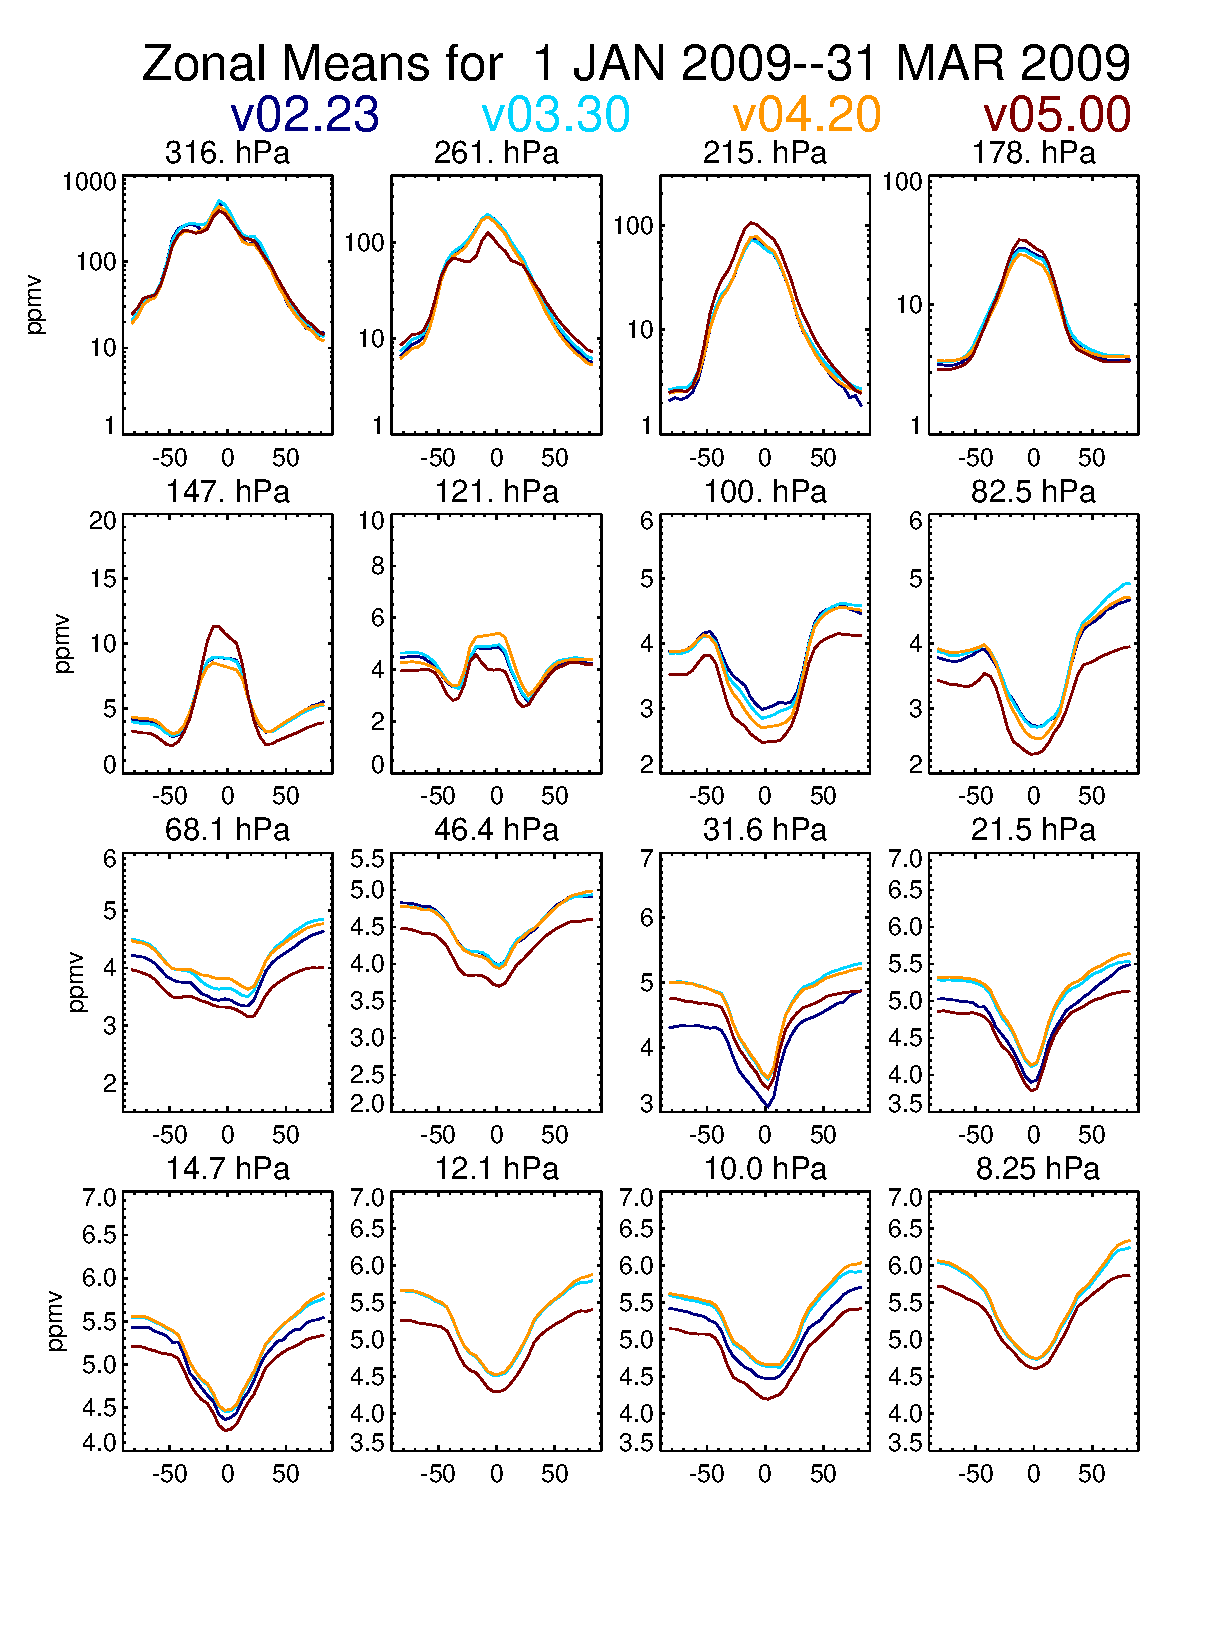
\includegraphics[width=0.8\linewidth]{figures/mls_h2o_v2-v3-v4-v5_zonal_means_ut-st}
\end{center}
\caption{A comparison of v2.23 (blue), v3.30 (cyan), v4.20 (orange), and v5.00
  (red), water vapor zonal means for Jan-Feb-Mar 2009. Each panel represents a
  pressure as noted above. The pressures shown range from 316~hPa to 8.3~hPa.}
\label{fig:avgmlsh2ozmcomp1}
\end{figure}

\begin{figure}
\begin{center}
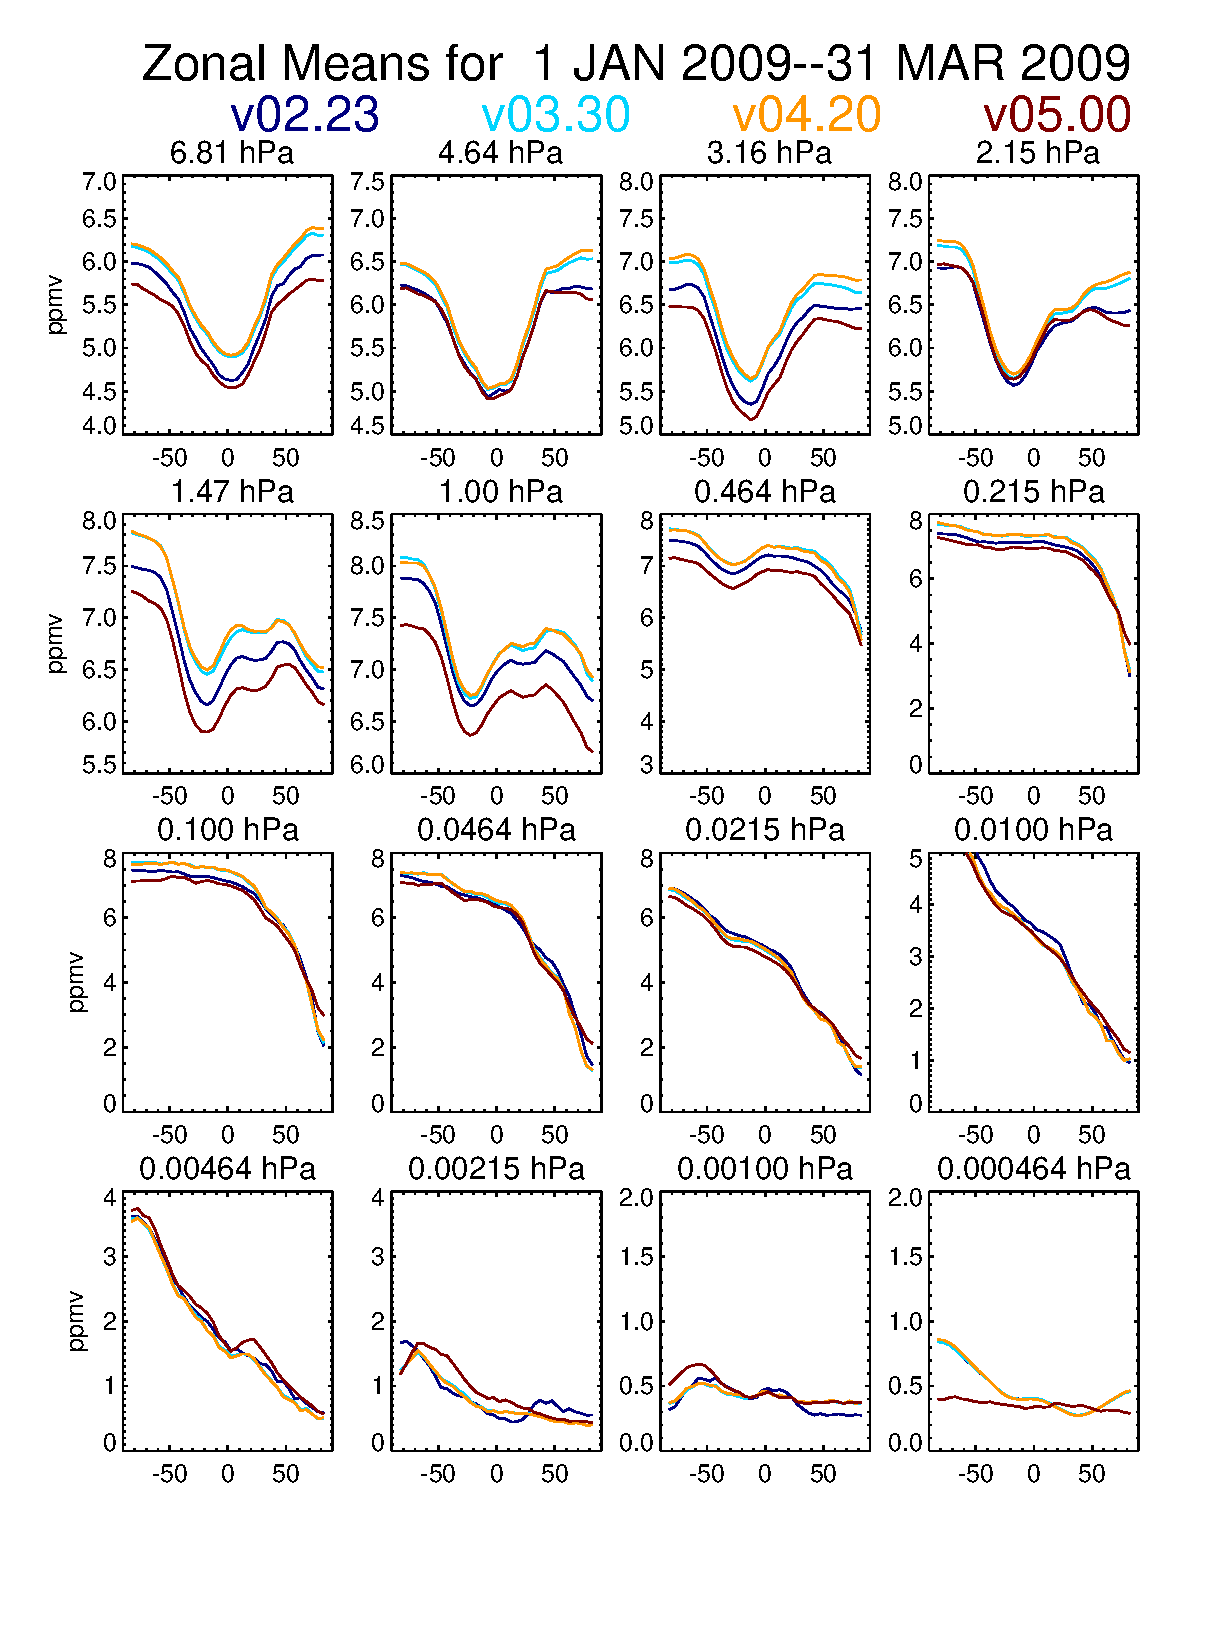
\includegraphics[width=0.8\linewidth]{figures/mls_h2o_v2-v3-v4-v5_zonal_means_usm}
\end{center}
\caption{A comparison of v2.23 (blue), v3.30 (cyan), v4.20 (orange), and v5.00
 (red) water vapor zonal means for Jan-Feb-Mar 2009. Each panel represents a
 pressure as noted above. The pressures shown range from 6.8\,hPa to
 0.00046\,hPa.}
\label{fig:avgmlsh2ozmcomp2}
\end{figure}

\subsection{Resolution}
\onestandardavk{H2O_HR}{H\cs2O}%

The spatial resolution is obtained from examination of the averaging
kernel matrices shown in Figure~\ref{fig:AvkH2O_HR}.  The vertical
resolution for H\cs2O is in the range 1.3\,--\,3.6\,km from
316\,--\,0.22\,hPa and degrades to 6\,--\,11\,km for pressures lower
than 0.22\,hPa. The along track horizontal resolution is
\texttildelow170\,--\,350\,km for pressures greater than 4.6\,hPa, and
degrades to 400\,--\,740\,km at smaller pressures. The resolutions in
Table~\ref{tab:H2OSummary} are a smoothed average of the equatorial and
70\degsym N values shown in Figure~\ref{fig:AvkH2O_HR}. The horizontal
cross-track resolution is 7\,km, the width of the MLS 190-GHz
field-of-view for all pressures. The longitudinal separation of the MLS
measurements is 10\degsym\,--\,20\degsym\ over middle and lower
latitudes, with much finer sampling in polar regions. The instrument
nominally scans to 0.001~hPa, therefore the retrieved value at 0.00046~hPa
is not vertically resolved and is effectively a column measurement from
0.001~hPa to the spacecraft with the H\cs2O profile values for
p $\le$ 0.000215~hPa fixed at \emph{a priori} values. The measurement
is only horizontally resolved.

\subsection{Precision}

Table~\ref{tab:H2OSummary} summarizes the estimated precision of the MLS
\thisv H\cs2O data. For pressures $\geq100$\,hPa, the precisions
given are the $1\sigma$ scatter about the mean of coincident comparison
differences, which are larger than the formal retrieval precisions
\citep{ReadEtal:2007}.  For pressures $\leq83$\,hPa the precisions are the
$1\sigma$ scatter of coincident ascending/descending MLS profile
differences \citep{LambertEtal:2007}.  The individual Level~2 precisions
are set to negative values or zero in situations when the retrieved
precision is larger than 50\% of the a priori precision -- an indication
that the data are biased toward the a priori value.

\subsection{Accuracy}

The values for accuracy are based primarily on two sources: comparisons
with validated instruments and a full systematic error analysis
performed on the MLS measurement system as described (for v2, but the
same approach will be used for \thisv) in \citet{ReadEtal:2007} and
\citet{LambertEtal:2007}. The results in Table~\ref{tab:H2OSummary}
are for \prevv because the analysis for \thisv is yet to be done; however,
it is expected that those for \thisv will be similar.
For pressures between 316\,--\,178\,hPa,
comparisons between AIRS v6 and MLS \thisv show $<20$\% agreement in the
zonal mean (MLS usually drier for low concentrations and wetter for high
concentrations) equatorward of 40\degsym\ with MLS having a dry
biases at higher latitudes.

The values in Table~\ref{tab:H2OSummary} for pressures between 316 and
178\,hPa are AIRS validated accuracies which are better than those
theoretically possible for the MLS measurement system. For the pressure
range 178\,--\,83\,hPa, the quoted values come directly from the
systematic error analysis performed on the MLS measurement
system. Comparisons between MLS and frost point hygrometers show that,
for the \prevv, when the tropopause is between 215 and 147\,hPa, MLS H\cs2O
2--3~km below the tropopause tends to have a large (20\,--\,40\%) dry bias.
It is anticipated that this dry bias will be reduced in \thisv but has yet
to be quantified. An estimate of the
accuracy between 121\,--\,83\,hPa is also from the systematic error
analysis performed on the MLS measurement system.  Comparisons among
\emph{in situ} sensors on the WB-57 high altitude aircraft and
frostpoint hygrometers flown on balloons show 30\% disagreements -- well
in excess of the estimated accuracy of each instrument including MLS --
near the tropopause and lower stratosphere.  The balloon based frost
point hygrometer shows agreement better than indicated in
Table~\ref{tab:H2OSummary}. The validation paper describes in detail why
a 30\% spread is inconsistent with the MLS measurements
\citep{ReadEtal:2007}.  For pressures less than 83\,hPa, the accuracy is
based on the systematic error analysis.

A long term drift in H\cs2O is being addressed in \thisv. It is believed
that a drift in the instrument sideband fraction is the cause and based on
opaque signals in the 190~GHz radiometer, can be evaluated and corrected.
More investigation will be done in the future to assess its performance.

\subsection{A note about the water vapor averaging kernels}

The averaging kernels are most applicable to linear and moderately
non-linear retrieval problems. The MLS H\cs2O retrievals are mostly
linear, except when the atmosphere approaches opaqueness. This occurs
when the limb tangent of the instrument field of view is less than
10\,km above the Earth's surface and the atmosphere is moist.  In such
cases the measurements are very nonlinear and often times the averaging
kernel calculations for the lowest retrieved levels are numerically
unstable, and unrepresentative of the actual MLS measurement system.
This is the case, for example, for the 316-hPa and 262-hPa equatorial
kernels shown in Figure~\ref{fig:AvkH2O_HR}.  Analysis of simulated MLS
observations indicates that application of the averaging kernel provides
little benefit to analyses involving the 316-hPa and 262-hPa levels, and
accordingly we recommend not applying the (unrepresentative) kernels at
those levels.

\subsection{Review of comparisons with other datasets}

\begin{figure}
\begin{center}
  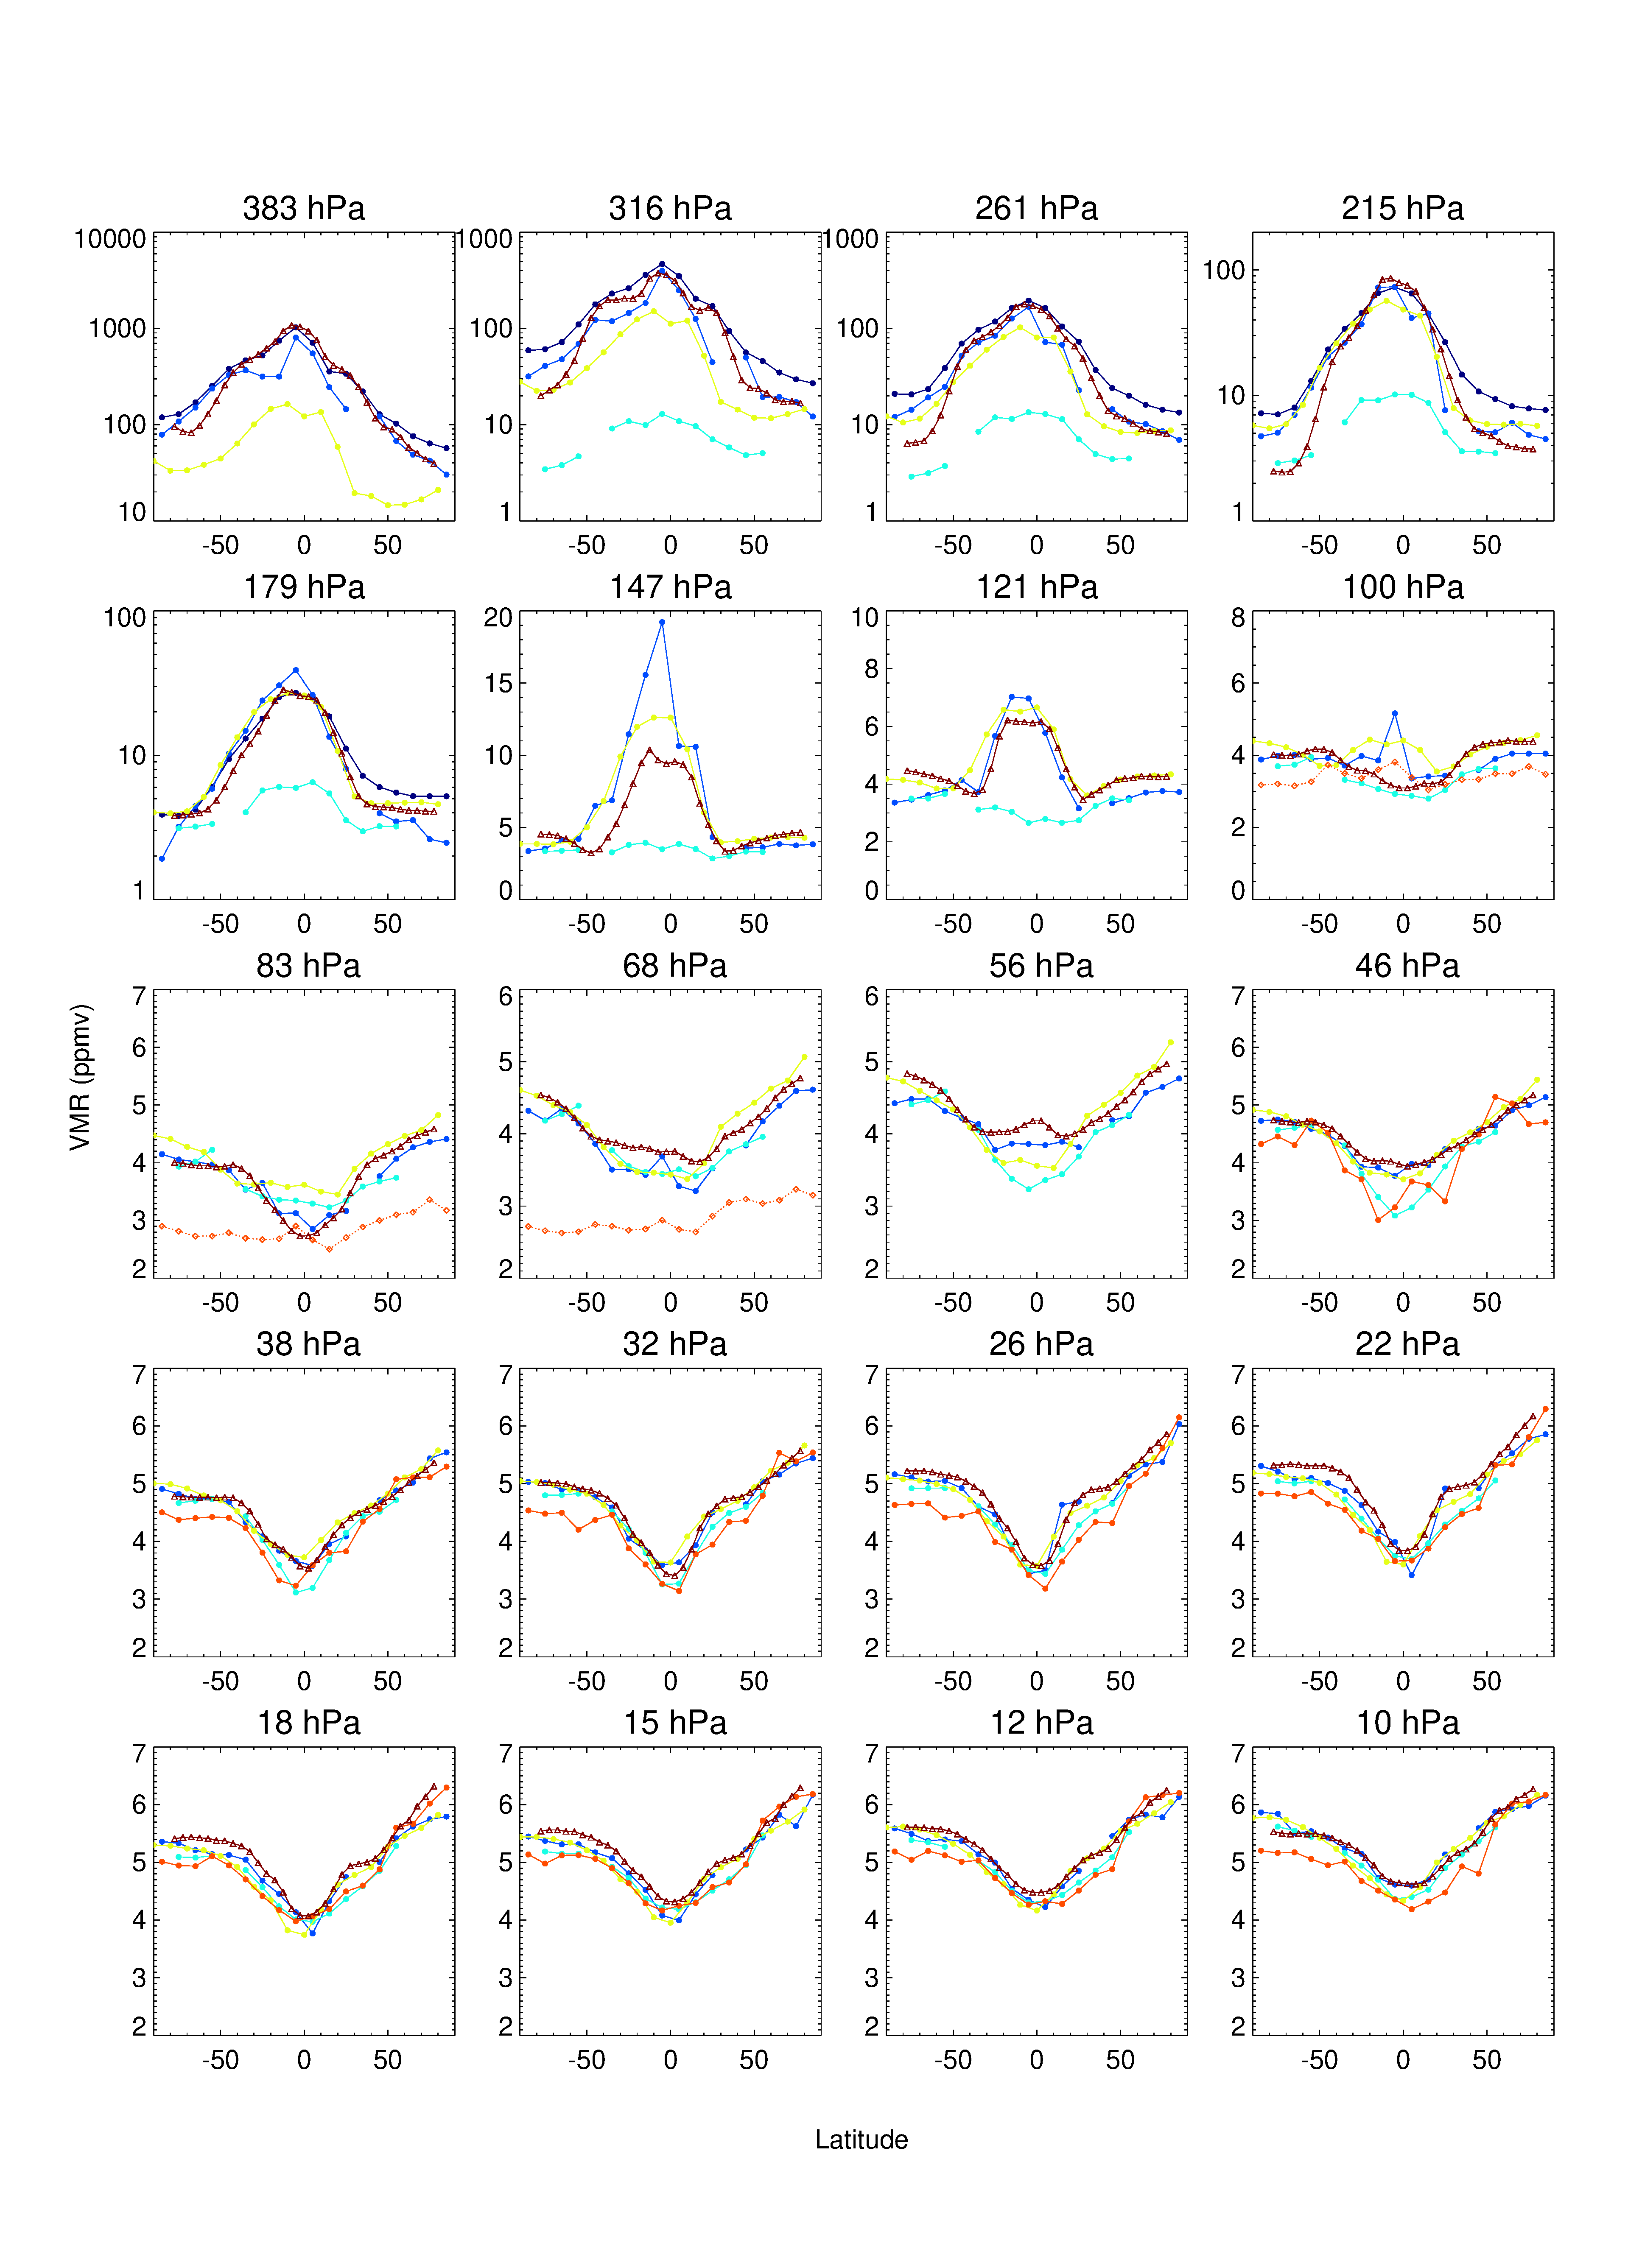
\includegraphics[bb = 58 120 1776 2340, clip, width=0.9\linewidth]{figures/sat_h2o_comps}
\end{center}
\caption{A comparison of MLS \thisv (red) water vapor for Jan-Feb-Mar
  2009 with other satellite observations shown as latitude-value zonal
  means. Each panel represents a pressure surface. The satellites are:
  AIRS v6 (dark blue), ACE-FTS v3.5 (light blue), MIPAS IMK v4
  (yellow-green), HALOE v19 (cyan), Odin SMR 544 GHz continuum product
  (orange open diamonds), and Odin SMR line resolved product (orange
  solid bullets).}
\label{fig:satcomps}
\end{figure}

Figure~\ref{fig:satcomps} shows a latitude-value zonal mean comparison
among several satellite data sets. The satellite datasets include MLS
\thisv, AIRS v6, ACE-FTS v3.5, MIPAS IMK v4, HALOE v19, Odin SMR
continuum H\cs2O, and Odin SMR line resolved H\cs2O. The data sets
show agreement for the stratospheric levels shown here beginning with
32~hPa and lower. More significant departures exist amongst them between
121--38~hPa even showing different latitude stucture. Averaging kernels
were not applied here because the nominal resolution of these datasets are
similar but each data set will exhibit its own vertical smoothing and
\emph{a priori} dependencies which is a contributing factor to the
differences where a sharp vertical gradient change at the tropopause occurs.
The patterns are more similar for the upper tropospheric levels (316--147~hPa).

One potential improvement in \thisv is shown in
Figures~\ref{fig:airsmlsjfm2009maps} and \ref{fig:airsmlsjja2009maps}
that compare multi-month maps of MLS with AIRS v6. The very moist
regions over the tropics in \prevv and \thisv are drier than in v2.2 and v3.3
for the higher pressure levels and in better agreement with AIRS.

\begin{figure}
\begin{center}
  \includegraphics[width=0.9\linewidth]
{figures/grid_maps_jfm2009_airsv6-mlsv2-3-4-5.png}
\end{center}
\caption{Mapped fields from AIRS v6 (left), MLS v2.2 (center-left), MLS
  v3.3 (center), MLS \prevv (center-right), and MLS \thisv (right) pressures
  between 300\,--150\,hPa for Jan-Feb-Mar 2009. The black-white lines indicate
  the tropopause where the region poleward is in the stratosphere.
  Note that the AIRS measurement is mostly suitable for H\cs2O greater than
  10\,ppmv.}
\label{fig:airsmlsjfm2009maps}
\end{figure}

\begin{figure}
\begin{center}
  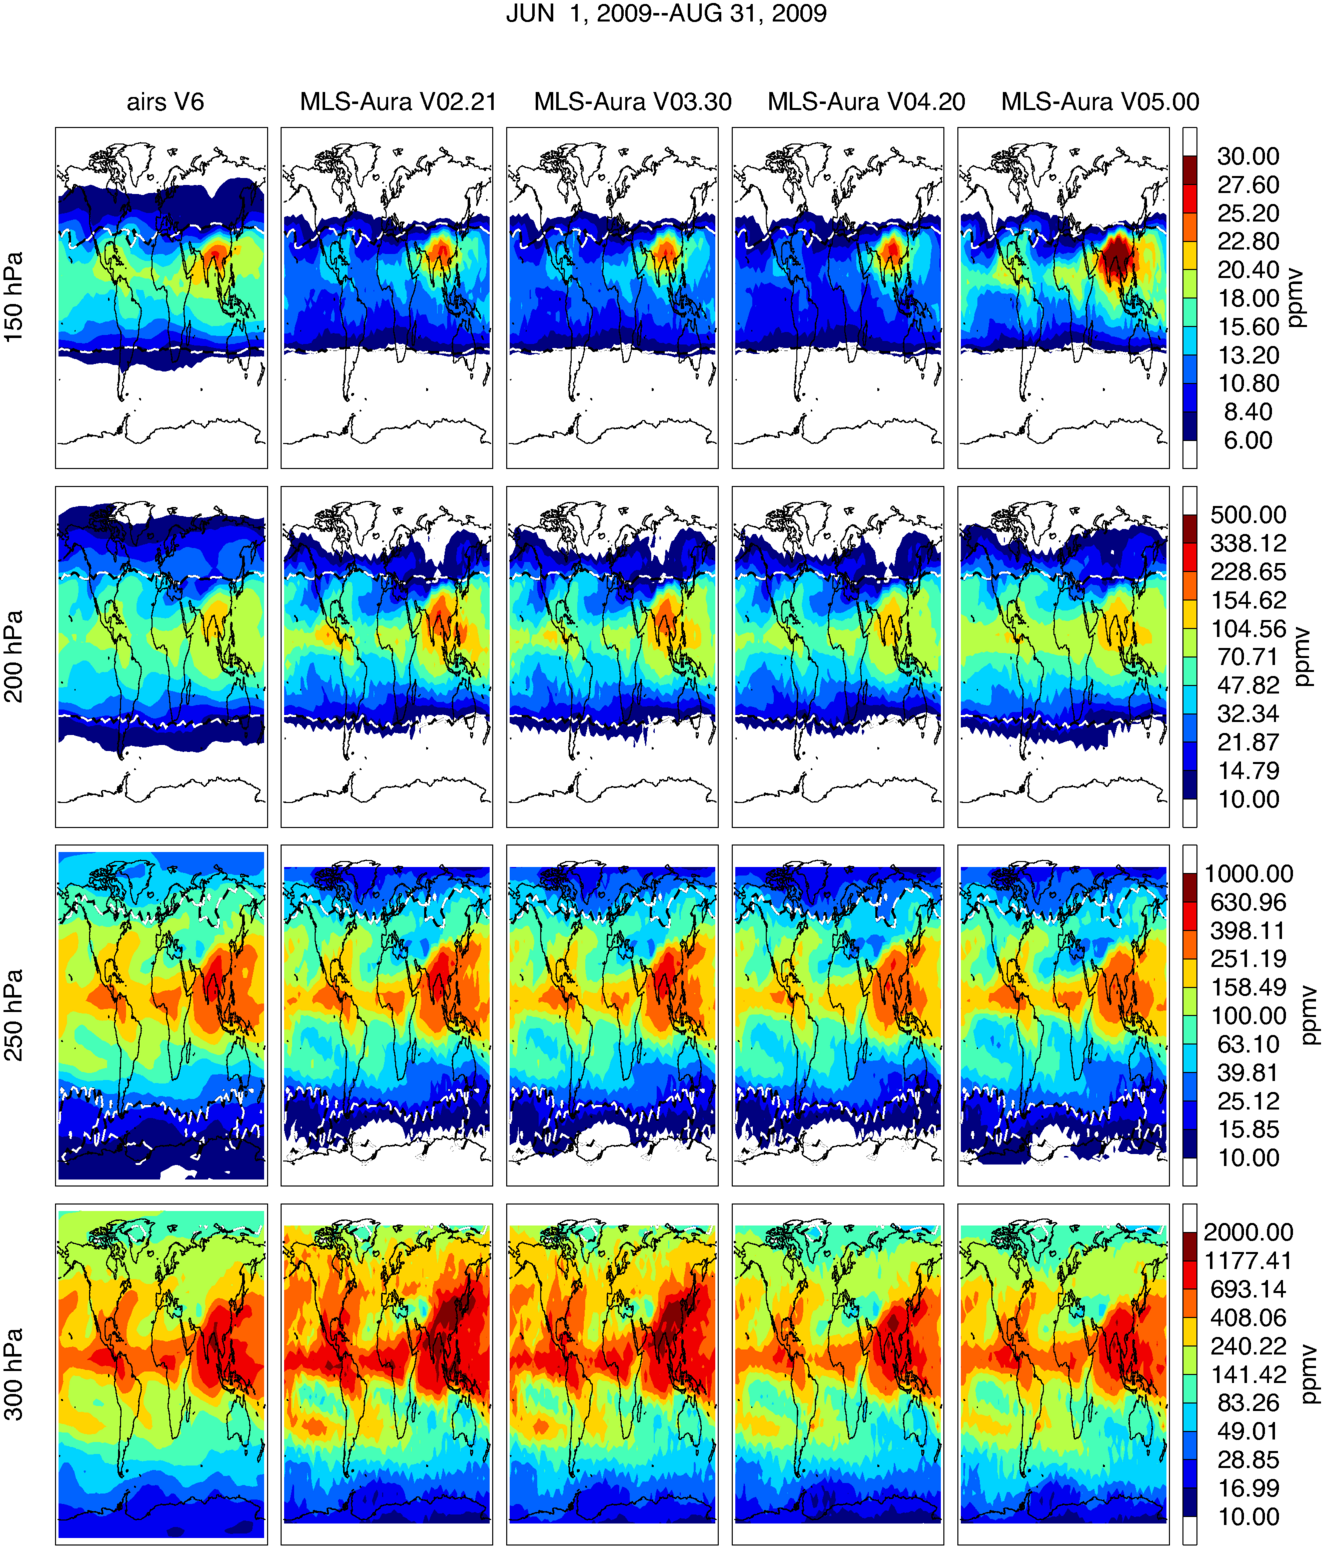
\includegraphics[width=0.9\linewidth]
{figures/grid_maps_jja2009_airsv6-mlsv2-3-4-5.png}
\end{center}
\caption{Mapped fields from AIRS v6 (left), MLS v2.2 (center-left), MLS
  v3.3 (center), MLS \prevv (center-right), and MLS \thisv (right) pressures
  between 300\,--\,150 hPa for Jun-Jul-Aug 2009. The black-white lines indicate
  the tropopause where the region poleward is in the stratosphere. 
  Note that the AIRS measurement is mostly suitable for H\cs2O greater than
  10\,ppmv.}
\label{fig:airsmlsjja2009maps}
\end{figure}

Apart from the differences noted above, the MLS \thisv H\cs2O is similar
to \prevv, v3.3, and v2.2 products, the latter described and
validated in \citet{ReadEtal:2007} and \citet{LambertEtal:2007}. The H\cs2O
validation paper used AIRS v4 and MLS v2 humidities and both of them
have become more dry in their subsequent versions. A revised validation
paper for H\cs2O is not planned in the near future and users are
encouraged to read \citet{ReadEtal:2007} and \citet{LambertEtal:2007} for more
information. MLS v4.2 is a part of the second SPARC Water Vapor
Assessment (WAVAS-II) activity.

\subsection{Potential drift in lower stratospheric water vapor}
\label{sec:H2ODrift}

Comparisons of lower stratospheric H\cs2O between MLS and balloon-borne CFH
and FPH\footnote{Cryogenic Frostpoint Hygrometer (CFH) and Frost Point
Hygrometer (FPH)} from 2004 to the present time show a drift in the agreement
with MLS water vapor increasing at a rate of
\mbox{0.03\,--\,0.07\,ppmv\,yr\cp{-1}} relative to the frostpoint sondes
(roughly 0.6 to 1.5\% per year), starting around 2009 \citet{HurstEtal:2016}.
Comparisons with the ACE-FTS instrument, and with measurements of upper
stratospheric water vapor from ground-based microwave sensors, provide
evidence for a smaller (\texttildelow+0.2\% per year) drift. The new
calibration values for the sideband fraction that are updated monthly are
yet smaller but approaching the drift seen with ACE-FTS but will significantly
underestimate the larger drift reported by \citeauthor{HurstEtal:2016}. A
complete assessment of the drift correction will have to wait until more
reprocessed data becomes available.

\subsection{Data screening}
\label{sec:H2OScreening}
\begin{description}
\item[Pressure range:] \screeningrule{316\,--\,0.00046\,hPa.}
  \standardrangestatement\,Using data at 0.00046\,hPa requires consultation
  with the MLS team.
\standardprecisionrule
\evenstatusrule
\item[Clouds:] Ignore status bit 16 (high cloud) or bit 32 (low cloud) set
indicating the presence of clouds. See artifacts for more details.
\item[Quality field:] \screeningrule{Only profiles with a value of the
    \texttt{Quality} \emph{greater} than 0.7 should be used in
    scientific studies.}  The quality threshold is deliberately set low
    because it is not a very good discriminator of poor profiles except when
    quality is well below the mean value; therefore,
    we recommend the ``additional screening to avoid outliers,'' as described
    below.
\item[Convergence field:] \screeningrule{Only profiles with a value of
    the \texttt{Convergence} \emph{less} than 2.0 should be used in
    scientific studies.}
\item[Additional screening to avoid outliers:] After application of
  the \texttt{Status}, \texttt{Quality}, and \texttt{Convergence}
  screening described above, there remain some unphysical profiles in
  the MLS \thisv\ H\cs2O dataset. These are characterized by
  unrealistically low water vapor mixing ratios in the upper troposphere
  and stratosphere. The cause behind this behavior is from using the
  logarithmic basis which excludes negative values. Sometimes the retreival
  minimizer seeks a negative value (at a given level and is almost always 
  accompanied with severe vertical profile oscillations) which is not
  allowed and therefore an optimal fit to the measurement signal is
  not achieved. H\cs2O profiles having values less than 0.101~ppmv
  (0.101$\times 10^{-6}$VMR) at any pressure at or higher than 1\,hPa
  (vertical levels 1--37) should not be used. Profiles with acceptable
  \texttt{status}, \texttt{quality}, and \texttt{convergence} with values
  less than 0.101~ppmv at pressures $<$ 1~hPa (vertical levels 38--55) are
  acceptable and occur frequently because the water vapor
  concentration in the mesosphere is often less than the measurement
  precision and negative values are preferable but not allowed due to the
  logarithmic basis definition being used.
 
\end{description}

\subsection{Artifacts}

There is a minimum concentration where MLS H\cs2O measurements become
unreliable. This is given in Table~\ref{tab:H2OSummary} under the ``Min.
H\cs2O'' column. The lowest allowable H\cs2O value is 0.1\,ppmv.
Differences between the retrieved middle tropospheric H\cs2O constraint
and the true atmospheric state can cause errors at 316 and 261\,hPa.
The error manifests either as dry ($<$1\,ppmv) or moist spikes in an
orbital time series. Such data are often accompanied with good quality
and status but is rejected by checking the profile for such events.

Clouds in the field of view degrade the data in unpredictable ways. Many
instances of quality $<$0.7 occur in the presence of clouds where the
cloud screening of the radiances failed to reject them. Cloud radiative
scattering distorts the spectral lineshape causing poor fits and low
quality values.  However, not all MLS signals are obviously
affected. Coincident comparisons of MLS cloud flagged H\cs2O
(\texttt{status} bit 16 or 32 set between 316\,--\,215\,hPa) having good
quality with AIRS show a small mean bias of 10\% but exhibit a 50\% increase
in variability for the individual differences. Therefore users should be
aware that, although the overall biases for measurements inside clouds
are similar to that for clear sky, individual profiles will exhibit
greater variability about the true atmospheric humidity.

The 190~GHz radiometer signals due to aging are drifting. This drift manifests
as a change in the sideband fraction. \thisv makes an attempt to correct this.

In the mesosphere, the precision is often larger than the
retrieved value and therefore negative concentrations are possible and
proper. The logarithmic definition of the H\cs2O basis doesn't allow retrieval
of negative values with the minimum lowest allowed concentration being 0.1~ppmv.
Therefore an average of many profiles will produce a positive bias. It is
recommended that a better representation of the average of many profiles is
achieved by calculating its median.

The instrument scan nomimnally tops out at 0.001~hPa. Therefore,
the 0.00046~hPa which is now retrieved in \thisv is not a vertically
resolved measurement but rather a column amount from 0.001~hPa to the
spacecraft under the constraint that all levels above 0.00046~hPa are fixed
at \emph{a priori} values. What this means is that should there be a large
H\cs2O event in any level above 0.00046~hPa would be retrieved as an
enhanced event at 0.00046~hPa but its vertical location above 0.00046~hPa is
unknown.

\subsection{Desired improvements for future data version(s)}

While many defects in v4.2 and earlier versions have been addressed,
futher investigation to their effectiveness, especially the drift
reduction and high latitude low value retrievals in the upper
troposphere needs to be assessed and improved upon if necessary.
Possibly a vertically resolved H\cs2O product for
pressure $>316\,\text{hPa}$ at high latitudes during dry conditions.

\begin{table}
\caption{Summary of MLS \thisv H\cs2O product.}
\vspace{\tablecaptionsep}
\label{tab:H2OSummary}
\begin{minipage}{\linewidth}
\centering\begin{tabular}{cccccm{30ex}}
\toprule
\parbox{10ex}{\centering\bfseries Pressure / hPa} &
\parbox{11ex}{\centering\bfseries Resolution V$\times$H / km} &
\parbox{10ex}{\centering\bfseries Precision\footnote{Precision for a
    single MLS profile} / \%} &
\parbox{10ex}{\centering\bfseries Accuracy / \%} &
\parbox{10ex}{\centering\bfseries Min. / ppmv\footnote{Minimum H\cs2O is an estimate of the minimum H\cs2O 
concentration measurable by \thisv MLS.}} &
\parbox{11ex}{\centering\bfseries Comments} \\
\midrule
$\le$0.00022  & --- & --- & --- & --- & Unsuitable for scientific use \\
0.0005 & NVR\footnote{Not Vertically resolved (NVR)}  $\times$ TBD & 900 &
TBD\footnote{Not yet determined} & 0.1 & Nominally a slant column measurement
for p $\le$ 0.001 hPa. \\
0.001 & TBD  $\times$ TBD &450 & TBD\footnote{Not yet determined} & 0.1 & \\
0.002 & 10.3 $\times$ 350 &152 & 40 & 0.1 & \\
0.005 & 10.8 $\times$ 585 & 81 & 23 & 0.1 & \\
0.010 &  8.8 $\times$ 725 & 55 & 17 & 0.1 & \\
0.022 &  8.0 $\times$ 745 & 41 & 19 & 0.1 & \\
0.046 &  7.4 $\times$ 540 & 35 & 17 & 0.1 & \\
0.10 &  5.8 $\times$ 745 & 24  & 14 & 0.1 & \\
0.22 &  3.6 $\times$ 670 & 19  & 11 & 0.1 & \\
0.46 &  3.3 $\times$ 505 & 12  &  8 & 0.1 & \\
1.0 &  2.5 $\times$ 400 &  6   &  7 & 0.1 & \\
2.2 &  3.5 $\times$ 385 &  4   &  7 & 0.1 & \\
4.6 &  3.4 $\times$ 350 &  4   &  5 & 0.1 & \\
10 &  2.8 $\times$ 290 &  6    & 19 & 0.1 & \\
22 &  3.2 $\times$ 265 &  5    &  5 & 0.1 & \\
46 &  3.2 $\times$ 230 &  5    &  4 & 0.1 & \\
68 &  3.1 $\times$ 190 &  5    &  9 & 0.1 & \\
83 &  3.1 $\times$ 190 &  7    &  9 & 0.1 & \\
100 & 3.0 $\times$ 198 & 15 &  8 & 0.1 & \\
121 & 2.6 $\times$ 193 & 20 & 12 & 0.1 & \\
147 & 2.3 $\times$ 188 & 20 & 15 & 0.1 & \\
178 & 1.7 $\times$ 183 & 25 & 20 & 3  & \\
\addlinespace
215 & 1.6 $\times$ 178 & 40  & 25 & 3   & Extent of a low bias for latitudes
$>60\degsym$ to be investigated. \\
\addlinespace
261 & 1.4 $\times$ 173 & 35  & 20 & 4   & Extent of low bias for latitudes
$>60\degsym$ to be invesrtigated. \\
\addlinespace
316 & 1.3 $\times$ 168 & 65  & 15 & 7   & Occasionally erroneous low value
$<1\,\text{ppmv}$ and high value fliers are retrieved in the tropics, usually in
clouds. \\
\addlinespace
$>316$ & --- & --- & --- & --- & Unsuitable for scientific use \\
\bottomrule
\end{tabular}
\end{minipage}
\end{table}


%%% Local Variables: 
%%% mode: latex
%%% TeX-master: "v5-x-report"
%%% End: 
